\documentclass[10pt]{article}

%%%%%%%%%%%%%%%%%%%%%%%%%%%%%%%%%%%%%%%%%%%%%%%%%%%%%%%%%%%%%%%%%%%%%%%%%%%%%%%
%%% packages %%%
%%%%%%%%%%%%%%%%%%%%%%%%%%%%%%%%%%%%%%%%%%%%%%%%%%%%%%%%%%%%%%%%%%%%%%%%%%%%%%%

\usepackage[english]{babel} % Choose english language
\usepackage[labelfont = bf, font = small]{caption} % Use caption package. Use bold font for caption.
\usepackage{siunitx} % Use siunitx for unit representation.
\newcommand{\RM}[1]{\MakeUppercase{\romannumeral #1{:}}}
\usepackage{graphicx}
\usepackage{tabularx}
\usepackage{float}
\usepackage{lmodern}
\usepackage{filecontents}
\usepackage{amsmath}
\usepackage{amssymb}
\usepackage[utf8]{inputenc}
\usepackage[bottom]{footmisc}
\usepackage{leftidx}
\usepackage{subcaption}
\usepackage[explicit]{titlesec}
\usepackage{booktabs}
\usepackage{multirow}
\usepackage{multicol}
\usepackage{listings}
\usepackage{pgfplots}
\usepackage{natbib}
\usepackage{xcolor}
\usepackage{url}
\usepackage{array}
\usepackage{setspace}
\usepackage{hyperref} % Referencing
\usepackage{verbatim}
\usepackage{changepage}
\usepackage[footnote, printonlyused]{acronym}
\usepackage{scrextend}
\usepackage{geometry} % Change geometry of page layout
\usepackage{rotating}
\usepackage{longtable}
\usepackage{lscape}
\usepackage{tocloft}
\usepackage{listings}
\usepackage{feynmp-auto} % Create fenynman diagrams
\usepackage{tikz-feynman} % Create fenynman diagrams
\usepackage{lipsum} % For testing. insert random text

%%%%%%%%%%%%%%%%%%%%%%%%%%%%%%%%%%%%%%%%%%%%%%%%%%%%%%%%%%%%%%%%%%%%%%%%%%%%%%%
%%% new commands and environments %%%
%%%%%%%%%%%%%%%%%%%%%%%%%%%%%%%%%%%%%%%%%%%%%%%%%%%%%%%%%%%%%%%%%%%%%%%%%%%%%%%

% Create custom font
\newenvironment{myfont}{\fontfamily{put}\selectfont}{\par}

% Adapt spacing between lines
\doublespacing

% Delete dots from toc
\renewcommand{\cftdot}{}

% Change section label to roman
\renewcommand{\thesection}{\Roman{section}}

% Customize section layout
\newcommand{\ssection}[1]{%
  \section[#1]{\centering\normalfont\scshape #1}}
\newcommand{\ssubsection}[1]{%
  \subsection[#1]{\centering\normalfont\itshape #1}}
\newcommand{\ssubsubsection}[1]{%
  \subsubsection[#1]{\centering\normalfont #1}}

% Import tikz libraries for figures
\usetikzlibrary{positioning,shadows,arrows}

% Create footnotereferencing
\makeatletter
\newcommand\footnoteref[1]{\protected@xdef\@thefnmark{\ref{#1}}\@footnotemark}
\makeatother

% Change layout of page
\hypersetup{
  colorlinks = true,
  linkbordercolor = {red},
  citebordercolor = {red},
  menubordercolor = {blue},
  urlbordercolor = {blue},
  linktoc = {page},
  pagebackref = {True},
  pdftitle = {Solution 04},
  pdfauthor = {Nils Hoyer, Maurice Morgenthaler},
  pdfcreator  = {pdflatex},
  pdfproducer = {LaTeX}
}

% Change geometry of page
\geometry{a4paper, top = 20mm, left = 20mm, right = 20mm, bottom = 15mm, headsep = 8mm, footskip = 10mm, includeheadfoot}

% Decalre uits for SIunitx
\DeclareSIUnit\femtobarn{fb^{-1}}

% Define colors
\definecolor{deepblue}{rgb}{0,0,0.5}
\definecolor{deepred}{rgb}{0.6,0,0}
\definecolor{deepgreen}{rgb}{0,0.6,0.2}
\definecolor{deeporange}{rgb}{0.9,0.2,0}

%%%%%%%%%%%%%%%%%%%%%%%%%%%%%%%%%%%%%%%%%%%%%%%%%%%%%%%%%%%%%%%%%%%%%%%%%%%%%%%
%%% start document %%%
%%%%%%%%%%%%%%%%%%%%%%%%%%%%%%%%%%%%%%%%%%%%%%%%%%%%%%%%%%%%%%%%%%%%%%%%%%%%%%%

\begin{document}
\begin{myfont}
\lstset{language=C++,
  basicstyle=\ttfamily,
  keywordstyle=\color{blue}\ttfamily,
  stringstyle=\color{red}\ttfamily,
  commentstyle=\color{green}\ttfamily,
  morecomment=[l][\color{magenta}]{\#}
}

\begin{center}
  \begin{Large}
    \textsc{Solution for homework assignment no. 04} \\
  \end{Large}
	\vspace*{0.4cm}
    Nils Hoyer, Maurice Morgenthaler
  \vspace*{1cm}
\end{center}

\section*{Exercise 4.1}

We are asked to write our own pseudo random number generator.
For this we will use the so called \textit{Blum Blum Shub} generator which uses the equation

\begin{equation}
n_{i+1} = n_{i}^{2} \;\%\; (p \cdot q)
\end{equation}

\noindent to generate new numbers.
$p$ and $q$ are large prime numbers. \\
To generate numbers between zero and one one has to divide by $p \cdot q$.

\begin{equation}
r_{i} = \frac{n_{i}}{M}
\end{equation}

\noindent Please find the code in file \texttt{exercise4\_1.C}.
The 20th 'random' numbers of consecitive seeds are listed in table \ref{tab:ex_1_results}.
Just by only looking at the twenty numbers below I can not see any correlation.

{\setstretch{1.0}
\begin{longtable}{*{2}l}
  \caption[]{The last twenty random numbers are listed given twenty consecutive seeds starting at \num{234509143}.}
  \endfirsthead
  \endhead
  \toprule
  \textbf{seed $i$} & \textbf{random number $r_{i}$} \\
  \midrule
  \num{234509143} & \num{0.38945} \\
  \num{234509144} & \num{0.05298} \\
  \num{234509145} & \num{0.55513} \\
  \num{234509146} & \num{0.31014} \\
  \num{234509147} & \num{0.82852} \\
  \num{234509148} & \num{0.53909} \\
  \num{234509149} & \num{0.41962} \\
  \num{234509150} & \num{0.10040} \\
  \num{234509151} & \num{0.15332} \\
  \num{234509152} & \num{0.45729} \\
  \num{234509153} & \num{0.53053} \\
  \num{234509154} & \num{0.47494} \\
  \num{234509155} & \num{0.01497} \\
  \num{234509156} & \num{0.32598} \\
  \num{234509157} & \num{0.90585} \\
  \num{234509158} & \num{0.01488} \\
  \num{234509159} & \num{0.68329} \\
  \num{234509160} & \num{0.25334} \\
  \num{234509161} & \num{0.46313} \\
  \num{234509162} & \num{0.90314} \\
  \bottomrule
  \label{tab:ex_1_results}
\end{longtable}}

\noindent Next we used the first seed to generate \num{10000} random numbers.
We filled a histogram with them which you can see in figure \ref{fig:ex_1_results}.

\begin{figure}[H]
  \centering
  \caption{\num{10000} random number generated by our own random number generator.
  The seed which has been used is \num{234509143}.
  We used \num{200} bins for plotting in the range between zero and one. \\
  Note that the rather large differences in amounts of numbers persists even to higher total numbers of generated 'random' numbers (e.g. \num{1000000}).}
  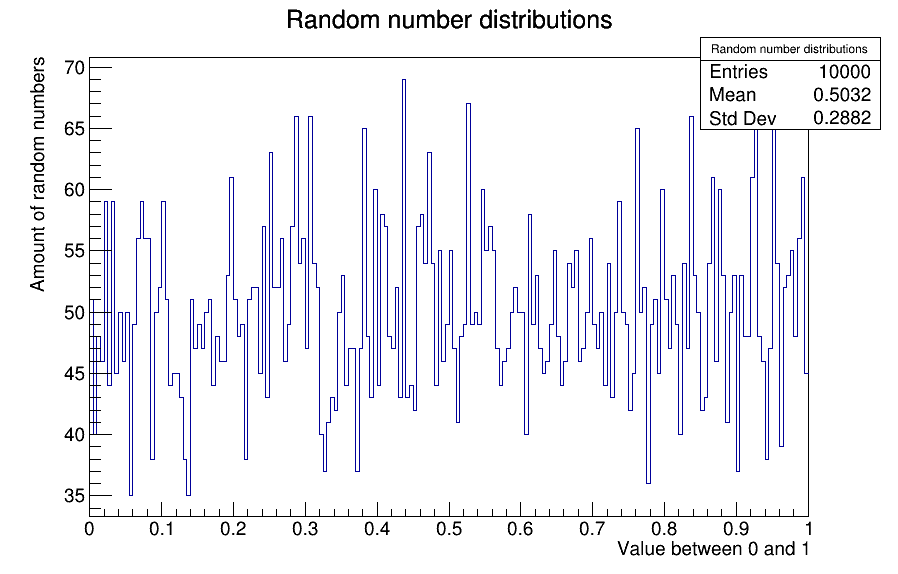
\includegraphics[width = \textwidth]{./canvas.png}
  \label{fig:ex_1_results}
\end{figure}

\end{myfont}
\end{document}